\chapter{Estudo de Caso}
\label{cap:estudo_caso_dev}

Este capítulo detalha a construção do estudo de caso prático, que se baseia no cenário de uma empresa fictícia e no desenvolvimento de uma plataforma de notícias sobre tecnologia, denominada ''WallTech''. Serão apresentados o contexto do projeto, os requisitos funcionais, a organização do processo de desenvolvimento, os métodos de design, a implementação das arquiteturas \acrshort{csr} e \acrshort{ssr}, e os testes comparativos realizados.

\section{Contexto}
\label{section:contexto}

Este estudo de caso parte do cenário de uma empresa fictícia do setor de notícias sobre tecnologia, cujo objetivo é fornecer conteúdos atualizados e relevantes sobre inovações e tendências do mercado. O público-alvo inclui entusiastas de tecnologia, profissionais da área e usuários que desejam acompanhar as novidades do setor em diferentes dispositivos, graças a uma interface responsiva.

A Figura \ref{fig:wireframe-walltech} apresenta o \textit{wireframe} da plataforma \textbf{WallTech}, gerado com o auxílio da ferramenta \textbf{V0.dev}, que utiliza inteligência artificial para criar protótipos de interfaces a partir de descrições textuais. Esse modelo visual orienta a organização dos elementos na interface antes da implementação das versões em \acrshort{csr} e \acrshort{ssr}.

\begin{figure}[H]
  \centering
  \caption{Wireframe da plataforma WallTech}
  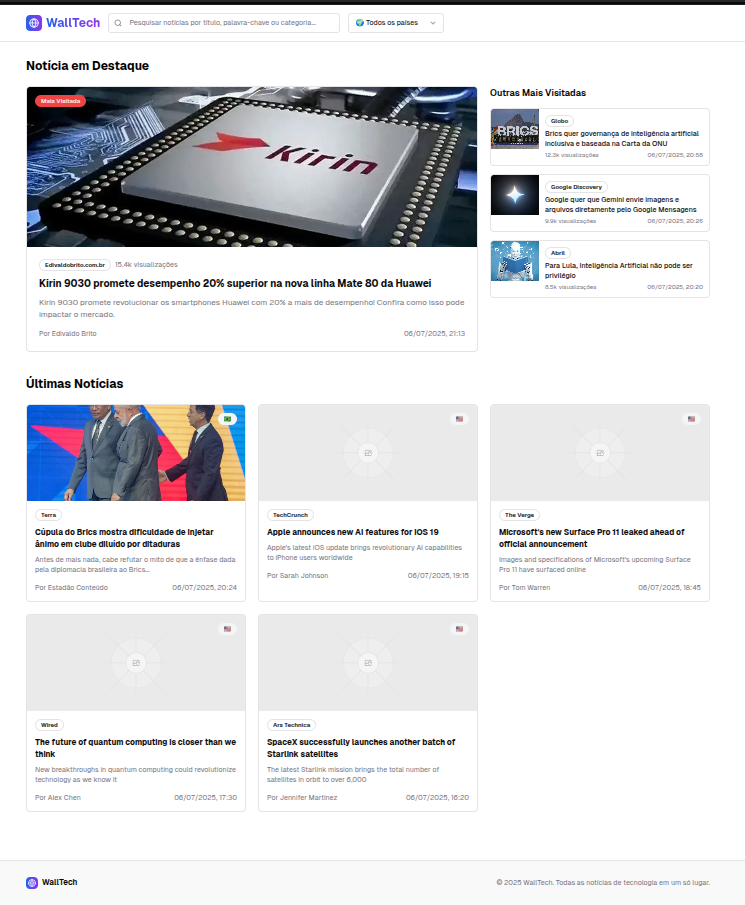
\includegraphics[width=0.7\textwidth]{media/wall_tech_wireframe.png}
  \legend{Fonte: os autores.}
  \label{fig:wireframe-walltech}
\end{figure}

Para analisar o impacto de diferentes abordagens de renderização web, foram desenvolvidos dois protótipos independentes da plataforma \textbf{WallTech}. O primeiro segue a abordagem de \acrfull{csr}, estruturado como uma \acrfull{spa} utilizando a biblioteca \textit{React}. O segundo utiliza \acrfull{ssr}, implementado como uma \acrfull{mpa} com o framework \textit{Next.js}.

A Figura \ref{fig:caso-uso-walltech} apresenta o diagrama de caso de uso da plataforma, destacando as principais funcionalidades acessíveis a usuários anônimos, como visualizar notícias recentes, acessar detalhes e realizar buscas por palavras-chave.

\begin{figure}[H]
  \centering
  \caption{Diagrama de caso de uso da plataforma WallTech}
  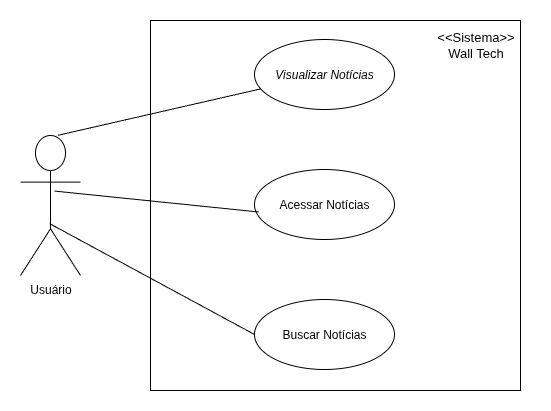
\includegraphics[width=0.7\textwidth]{media/wall_tech_use_case.png}
  \legend{Fonte: os autores.}
  \label{fig:caso-uso-walltech}
\end{figure}


\section{Processo de Desenvolvimento}
\label{section:processo-desenvolvimento}
O processo de desenvolvimento utilizado para construir a plataforma WallTech segue a metodologia ágil \english{Kanban}. Essa metodologia de desenvolvimento ágil é baseada em um quadro de tarefas, no qual cada tarefa é representada por um cartão \cite{gomes2014kanban}. O quadro Kanban é dividido em colunas que representam o estado atual de cada tarefa. As colunas mais comuns são: \english{To Do}, \english{In Progress} e \english{Done}, e o quadro é atualizado conforme as tarefas são realizadas. Além dessas colunas, o processo foi adaptado para incluir colunas adicionais como \english{Docs} e \english{Test}, permitindo que a documentação e os testes fossem gerenciados de forma organizada e eficiente durante o desenvolvimento.

A Figura \ref{fig:kanban-walltech} apresenta um exemplo do quadro Kanban utilizado no \english{GitHub Projects}, mostrando a organização das tarefas e o progresso do desenvolvimento da plataforma WallTech. O quadro reflete a estrutura de colunas adaptada, proporcionando uma visão clara do fluxo de trabalho da equipe, o que facilita o acompanhamento das tarefas em diferentes estágios.

Após a definição das funcionalidades principais do sistema, as tarefas foram inicialmente documentadas como \english{user stories}. As \english{user stories} são descrições simples e compreensíveis das funcionalidades a serem implementadas, permitindo uma comunicação clara entre a equipe de desenvolvimento e as partes interessadas. Cada \english{user story} é associada a um conjunto de requisitos específicos e uma definição de pronto, facilitando a compreensão do que precisa ser desenvolvido.

A partir dessas \english{user stories}, as \english{issues} foram criadas no \english{GitHub Projects}. Cada \english{issue} representa uma tarefa específica que deve ser realizada, baseada nas \english{user stories}. No \english{GitHub Projects}, essas \english{issues} são organizadas nas colunas do quadro Kanban, permitindo que a equipe visualize o progresso de cada tarefa e as mova conforme o andamento do trabalho.

A Figura \ref{fig:kanban-userstories} mostra um exemplo de cartão \english{issue} no \english{GitHub Projects}, ilustrando como as \english{user stories} são transformadas em tarefas e organizadas dentro do quadro Kanban. Cada \english{issue} possui detalhes sobre a tarefa, como descrições, prioridade e prazo, facilitando o gerenciamento e a execução das atividades no time de desenvolvimento.

\begin{figure}[H]
  \centering
  \caption{Exemplo de quadro Kanban no \english{GitHub Projects}}
  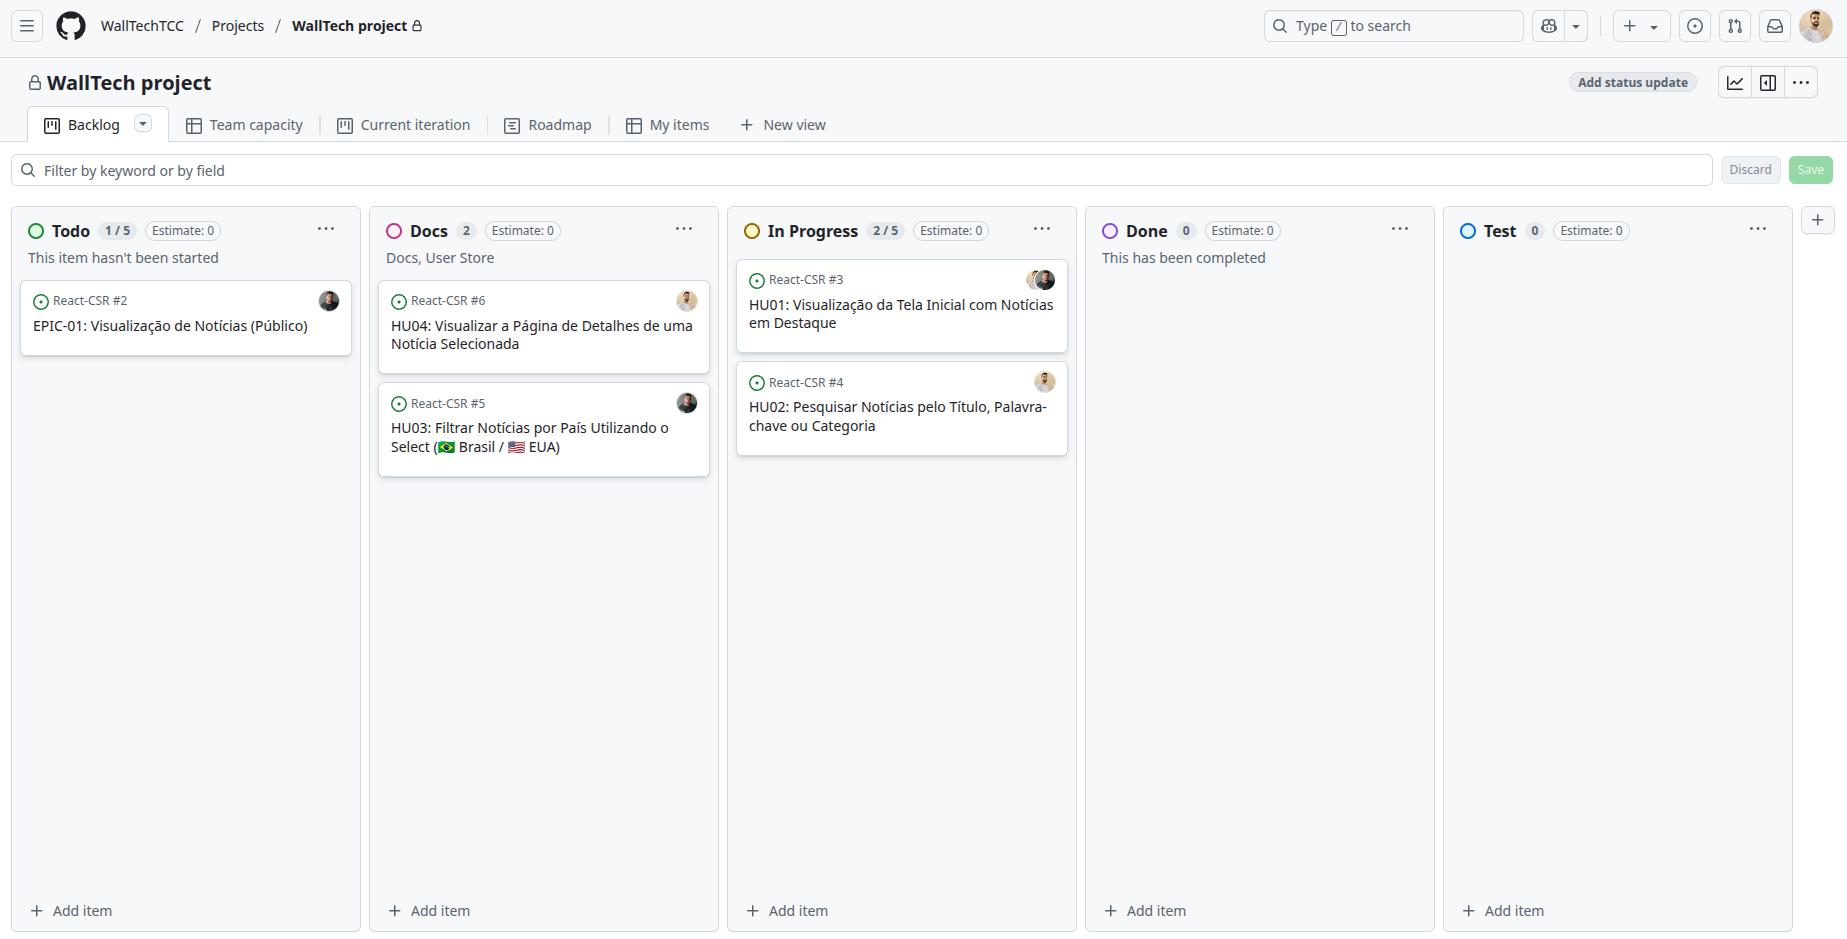
\includegraphics[width=1.0\textwidth]{media/wall_tech_kanban.png}
  \legend{Fonte: os autores.}
  \label{fig:kanban-walltech}
\end{figure}

\begin{figure}[H]
  \centering
  \caption{Exemplo de cartão \english{issue} no \english{GitHub Projects}}
  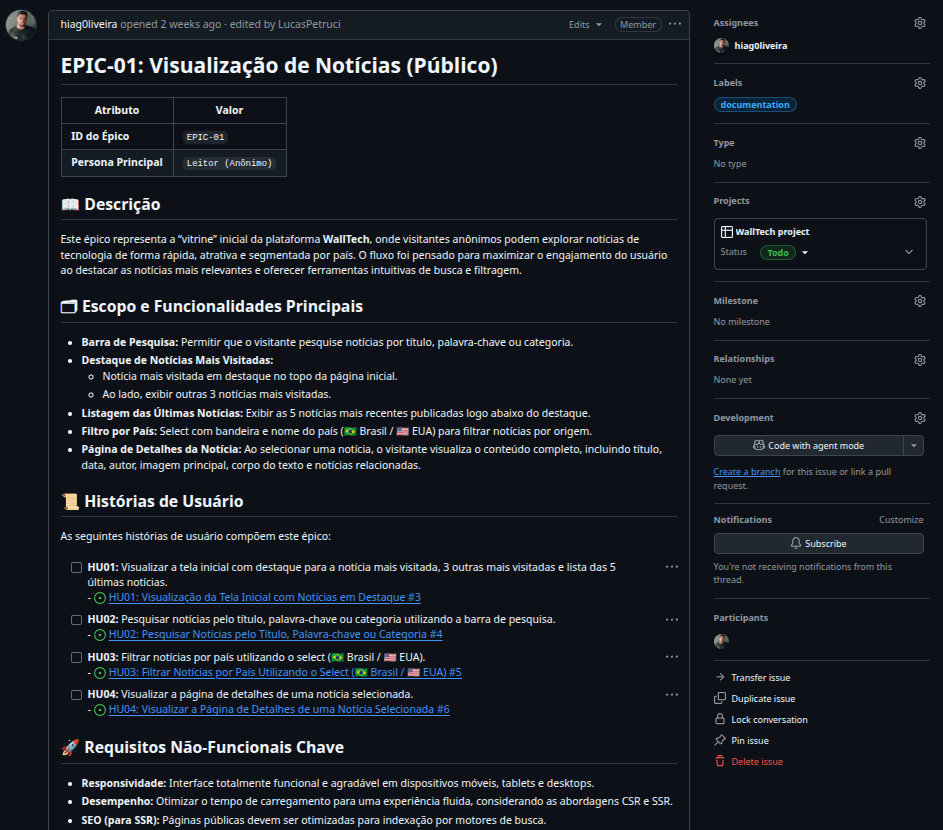
\includegraphics[width=0.7\textwidth]{media/wall_tech_epic.png}
  \legend{Fonte: os autores.}
  \label{fig:kanban-userstories}
\end{figure}




\subsection{Planejamento Funcional: Épico e Histórias de Usuário}

Para guiar o desenvolvimento da plataforma WallTech, foi adotada uma abordagem baseada em práticas ágeis, especialmente no uso de \textit{épicos} e \textit{histórias de usuário}. Essa técnica visa descrever funcionalidades a partir da perspectiva do usuário, proporcionando clareza sobre o propósito e os objetivos de cada componente da aplicação.

As histórias de usuário foram redigidas segundo o modelo dos 3Ws (Who, What, Why), uma técnica comum em análise de requisitos que busca responder:
\begin{itemize}
  \item \textbf{Who (Quem):} Quem está solicitando ou interagindo com a funcionalidade?
  \item \textbf{What (O quê):} Qual é a ação ou funcionalidade desejada?
  \item \textbf{Why (Por quê):} Qual é o benefício ou valor esperado para o usuário?
\end{itemize}

Esse modelo torna a narrativa mais centrada no usuário e contribui para um entendimento compartilhado entre desenvolvedores, designers e partes interessadas. Além disso, as funcionalidades foram agrupadas em épicos, que representam blocos de funcionalidades coesas e de maior escala dentro do sistema.

A seguir, apresenta-se o \textbf{EPIC-01}, responsável por organizar as funcionalidades relacionadas à visualização pública de notícias na plataforma WallTech, seguido de suas respectivas histórias de usuário.

\subsubsection*{EPIC-01: Visualização de Notícias (Público)}

\begin{itemize}
  \item \textbf{ID do Épico:} EPIC-01
  \item \textbf{Persona Principal:} Leitor (Anônimo)
\end{itemize}

\noindent \textbf{Descrição:} Este épico representa a “vitrine” da plataforma WallTech, onde visitantes anônimos podem explorar notícias de tecnologia de forma rápida, atrativa e segmentada por país. O fluxo foi pensado para maximizar o engajamento do usuário ao destacar as notícias mais relevantes e oferecer ferramentas intuitivas de busca e filtragem.

\noindent \textbf{Funcionalidades Principais:}
\begin{itemize}
  \item Barra de pesquisa (por título, palavra-chave ou categoria);
  \item Destaque para a notícia mais visitada e outras três recentemente acessadas;
  \item Listagem das cinco últimas notícias;
  \item Filtro por país (Brasil ou EUA);
  \item Página de detalhes da notícia com conteúdo completo e relacionadas.
\end{itemize}

\noindent \textbf{Requisitos Não-Funcionais:}
\begin{itemize}
  \item Interface responsiva em diferentes dispositivos;
  \item Otimização de desempenho para carregamento rápido;
  \item Suporte a SEO nas páginas públicas (relevante em SSR).
\end{itemize}

\noindent \textbf{Critérios de Aceite:}
\begin{itemize}
  \item Visitantes conseguem navegar e visualizar notícias sem necessidade de login;
  \item É possível realizar pesquisas e aplicar filtros por país;
  \item A navegação é responsiva, intuitiva e eficiente;
  \item A página de detalhes apresenta informações completas da notícia.
\end{itemize}

\subsubsection*{HU01: Visualização da Tela Inicial com Notícias em Destaque}

\begin{itemize}
  \item \textbf{Who:} Visitante anônimo
  \item \textbf{What:} Ver na página inicial uma barra de pesquisa, uma notícia mais visitada em destaque, três outras recém acessadas e uma lista com as cinco últimas notícias publicadas.
  \item \textbf{Why:} Explorar rapidamente o conteúdo mais relevante e recente sobre tecnologia.
\end{itemize}

\noindent \textbf{História:} \textit{Como um visitante, quero ver na página inicial uma barra de pesquisa, a notícia mais visitada em destaque, outras três recém visitadas ao lado e as cinco últimas notícias abaixo, para que eu possa explorar rapidamente o conteúdo mais relevante sobre tecnologia.}

\noindent \textbf{Critérios de Aceite:}
\begin{itemize}
  \item A página inicial contém uma barra de pesquisa funcional;
  \item A notícia mais visitada aparece em destaque;
  \item Outras três notícias aparecem ao lado da principal;
  \item Abaixo, as cinco últimas notícias são exibidas em ordem cronológica;
  \item Interface é responsiva e com bom desempenho.
\end{itemize}

\subsubsection*{HU02: Pesquisar Notícias por Palavra-chave ou Categoria}

\begin{itemize}
  \item \textbf{Who:} Visitante
  \item \textbf{What:} Utilizar a barra de pesquisa para buscar por título, palavra-chave ou categoria.
  \item \textbf{Why:} Encontrar conteúdos relevantes de forma eficiente.
\end{itemize}

\noindent \textbf{História:} \textit{Como um visitante, quero pesquisar notícias por título, palavra-chave ou categoria, para que eu possa encontrar facilmente conteúdos relevantes sem precisar navegar por toda a lista.}

\noindent \textbf{Critérios de Aceite:}
\begin{itemize}
  \item Campo de texto para busca;
  \item Filtro por categoria;
  \item Resultados relevantes são exibidos com base na busca;
  \item A busca pode ser combinada com o filtro por categoria;
  \item Mensagem amigável exibida em caso de nenhum resultado.
\end{itemize}

\subsubsection*{HU03: Filtrar Notícias por País}

\begin{itemize}
  \item \textbf{Who:} Visitante
  \item \textbf{What:} Filtrar as notícias por país usando um seletor com bandeiras.
  \item \textbf{Why:} Visualizar conteúdos específicos da localidade desejada.
\end{itemize}

\noindent \textbf{História:} \textit{Como um visitante, quero filtrar notícias por país (Brasil ou EUA), para que eu possa visualizar apenas conteúdos relevantes para minha localidade ou interesse regional.}

\noindent \textbf{Critérios de Aceite:}
\begin{itemize}
  \item Menu com seleção de país exibindo bandeira e nome;
  \item Lista de notícias é atualizada dinamicamente conforme a seleção;
  \item O filtro mantém o estado ao navegar;
  \item Filtro compatível com busca por palavra-chave ou categoria.
\end{itemize}

\subsubsection*{HU04: Visualizar Detalhes de uma Notícia}

\begin{itemize}
  \item \textbf{Who:} Visitante
  \item \textbf{What:} Acessar a página de detalhes de uma notícia específica.
  \item \textbf{Why:} Ler o conteúdo completo e visualizar informações adicionais.
\end{itemize}

\noindent \textbf{História:} \textit{Como um visitante, quero clicar em uma notícia para acessar sua página de detalhes, para que eu possa ler o conteúdo completo e visualizar informações relacionadas.}

\noindent \textbf{Critérios de Aceite:}
\begin{itemize}
  \item Acesso a uma URL única da notícia;
  \item Exibição completa do conteúdo (título, autor, data, imagem, corpo do texto, país de origem);
  \item Exibição de até três notícias relacionadas;
  \item Página de erro amigável no caso de URL inválida;
  \item Botão para retornar à lista ou pesquisa anterior.
\end{itemize}









\section{Requisitos}
\label{section:requisitos}

O levantamento e a definição dos requisitos da plataforma WallTech foram guiados pelas necessidades dos usuários e organizados por meio da técnica de \textit{histórias de usuário}, agrupadas em \textit{épicos}. A partir da análise funcional do \textbf{EPIC-01 — Visualização de Notícias (Público)}, foram identificadas as principais funcionalidades esperadas para a aplicação, considerando tanto o fluxo de interação do visitante quanto os objetivos de usabilidade, desempenho e escalabilidade.

A seguir, são apresentados os requisitos funcionais, que representam as funcionalidades diretamente percebidas pelos usuários, e os não funcionais, que tratam de atributos como desempenho, acessibilidade e responsividade.

\textbf{Requisitos Funcionais:}
\begin{itemize}
  \item O sistema deve permitir que visitantes visualizem uma lista de notícias recentes e em destaque.
  \item O sistema deve disponibilizar uma barra de pesquisa por palavra-chave, título ou categoria.
  \item O sistema deve permitir a filtragem de notícias por país (🇧🇷 Brasil ou 🇺🇸 EUA).
  \item O sistema deve possibilitar o acesso aos detalhes completos de uma notícia selecionada.
  \item O sistema deve armazenar localmente os acessos recentes para melhorar a experiência do usuário.
  \item O sistema deve apresentar mensagens claras em situações de ausência de conteúdo.
\end{itemize}

\textbf{Requisitos Não Funcionais:}
\begin{itemize}
  \item A interface deve ser responsiva, adaptando-se corretamente a diferentes tamanhos de tela.
  \item O carregamento das páginas deve ser otimizado, proporcionando uma experiência fluida mesmo em conexões lentas.
  \item O sistema deve estar preparado para indexação por motores de busca (SEO), quando aplicado via Server-Side Rendering.
  \item A navegação deve ser acessível, com suporte a teclado e leitores de tela.
  \item A interface deve manter a consistência visual e funcional entre suas versões SPA e MPA.
\end{itemize}




\section{Design do Sistema}
\label{cap:design}

O design do sistema foi orientado para refletir as diferenças estruturais entre as abordagens \acrshort{spa} e \acrshort{mpa}, levando em consideração os requisitos funcionais da plataforma \textit{WallTech}. Esta vitrine digital exibe notícias de tecnologia obtidas por meio da \textit{NewsAPI}, com recursos de busca, filtragem e destaque de conteúdo segmentado por país. Não há backend próprio, sendo todas as chamadas feitas diretamente para a API externa, o que simplifica a arquitetura e acentua o papel do frontend na renderização de conteúdo.

Para modelagem arquitetural e comportamental, foram utilizados diagramas da UML, incluindo:
\begin{itemize}
  \item \textbf{Diagrama de Caso de Uso}, para representar as principais funcionalidades acessadas pelos usuários visitantes.
  \item \textbf{Diagrama de Sequência}, a fim de ilustrar o fluxo de interação entre navegador e a \textit{NewsAPI} durante operações como busca e carregamento de notícias.
  \item \textbf{Diagrama de Componentes}, para representar os módulos da aplicação, como a interface, o serviço de requisição à API, e os componentes de renderização.
\end{itemize}

As decisões de design foram fundamentadas em boas práticas para renderização web discutidas por \cite{osmani2025}, bem como nas diretrizes da literatura especializada em arquitetura de frontend, como apresentado pela \cite{atori2024}.

Segundo \cite{osmani2025}, a escolha entre renderização no cliente ou no servidor deve considerar o contexto da aplicação, os requisitos de desempenho e os objetivos de SEO. Já o artigo da \cite{atori2024} destaca que SPAs tendem a oferecer maior fluidez e interatividade, enquanto MPAs são mais eficazes em aplicações que dependem de indexação e acessibilidade.

\section{Abordagens de Renderização e Navegação}
\label{section:abordagens-renderizacao}

Para o estudo comparativo, a plataforma foi desenvolvida em duas arquiteturas distintas de renderização e navegação: 
\acrfull{ssr} com \acrfull{mpa} e \acrfull{csr} com \acrfull{spa}.  
Cada abordagem foi implementada com tecnologias adequadas ao seu paradigma Next.js para \acrshort{ssr}/\acrshort{mpa} e React para \acrshort{csr}/\acrshort{spa}  permitindo observar diferenças de desempenho, interatividade e otimização para mecanismos de busca (\acrshort{seo}).

A seguir, cada abordagem é apresentada com seu fluxo típico de funcionamento, diagrama de componentes (representando a estrutura modular) e diagrama de sequência (detalhando as interações passo a passo).

\subsection{SSR/MPA - Fluxo e Arquitetura}
\label{subsec:ssr-mpa}

Na abordagem \acrfull{ssr} com \acrfull{mpa}, cada página é renderizada no servidor a partir de uma requisição HTTP completa. O HTML final já é entregue com os dados integrados, permitindo que o navegador exiba o conteúdo imediatamente, favorecendo o tempo de carregamento inicial e a indexação por \textit{crawlers} \cite{atori2024}.

\begin{itemize}
  \item O usuário acessa o site;
  \item O navegador envia uma requisição \texttt{GET} ao servidor Next.};
  \item O servidor obtém os dados mais recentes na NewsAPI;
  \item O servidor monta a página HTML já com os dados;
  \item O HTML é enviado ao navegador e exibido;
  \item Cada navegação subsequente gera nova requisição completa ao servidor;
  \item Scripts no cliente utilizam LocalStorage para melhorar a experiência.
\end{itemize}
  
A Figura \ref{fig:component-diagram-next} ilustra como, nesta arquitetura, o navegador interage diretamente com o Servidor Next.js para cada página requisitada. O servidor, por sua vez:

\begin{enumerate}
  \item Identifica a rota usando o roteamento baseado em arquivos;
  \item Executa a lógica de busca de dados (\texttt{getServerSideProps});
  \item Faz chamadas à NewsAPI para obter o conteúdo;
  \item Renderiza o HTML e o envia ao cliente.
\end{enumerate}

A Figura \ref{fig:sequence-diagram-ssr} detalha a ordem das interações. O usuário inicia a navegação, o servidor processa a requisição, consulta a API externa, renderiza o HTML e envia a resposta pronta para o cliente. O uso de \textit{hydration} ativa a interatividade após o carregamento inicial.

\begin{figure}[H]
  \centering
  \caption{Diagrama de sequência - \acrshort{ssr}/\acrshort{mpa}}
  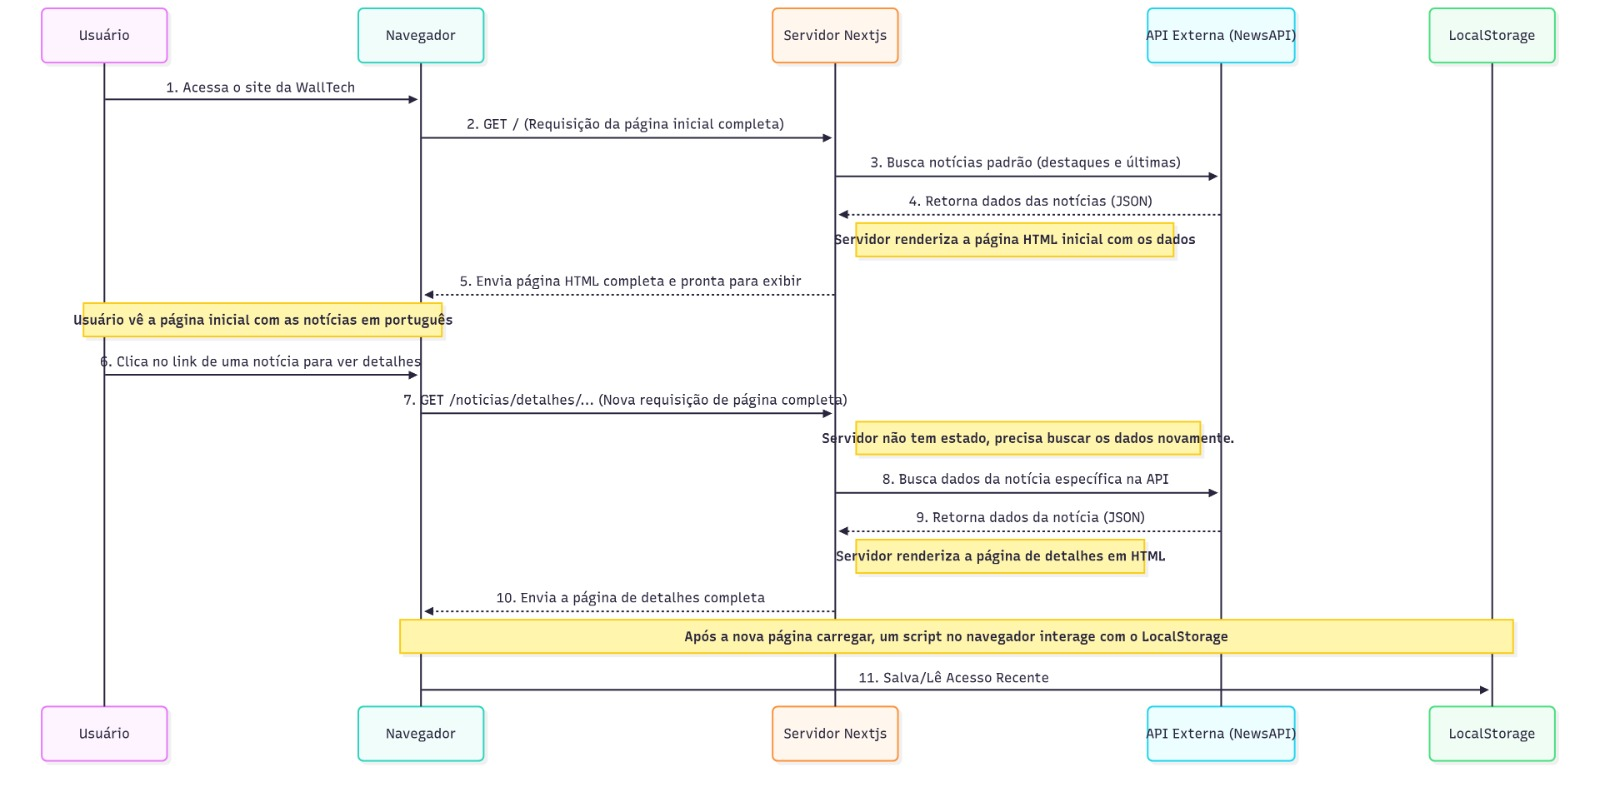
\includegraphics[width=1\textwidth]{media/wall_tech_sequence_diagram.jpeg}
  \legend{Fonte: os autores.}
  \label{fig:sequence-diagram-ssr}
\end{figure}

A Figura \ref{fig:component-diagram-next} mostra que, nessa arquitetura, o servidor Next.js centraliza o roteamento, a obtenção de dados e a renderização das páginas, entregando ao navegador HTML já pré-renderizado. Após o carregamento, scripts ativam a interatividade e permitem o uso do LocalStorage, uma interface da Web Storage API que possibilita armazenar dados no formato chave-valor de forma persistente no navegador do usuário, ideal para guardar informações como o histórico de notícias acessadas.


\begin{figure}[H]
  \centering
  \caption{Diagrama de Componentes - \acrshort{mpa} (\acrshort{ssr} em Next.js)}
  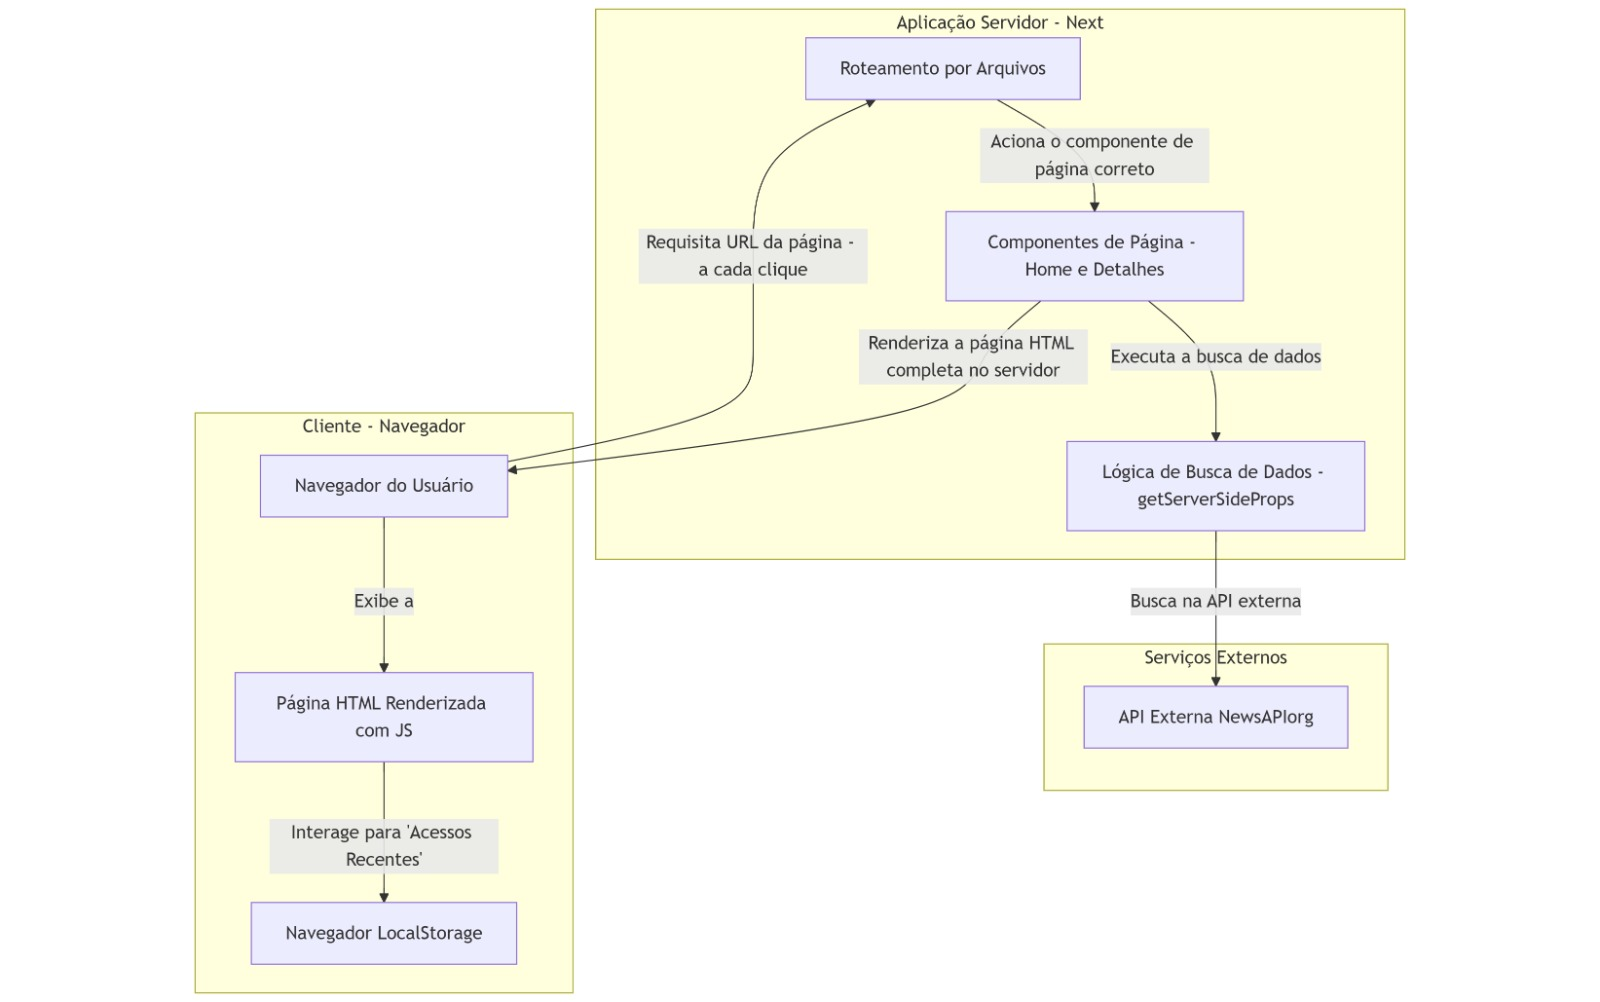
\includegraphics[width=1\textwidth]{media/component-diagram-next.jpeg}
  \legend{Fonte: os autores.}
  \label{fig:component-diagram-next}
\end{figure}


\subsection{CSR/SPA - Fluxo e Arquitetura}
\label{subsec:csr-spa}

Na abordagem \acrfull{csr} com \acrfull{spa}, o carregamento inicial envia um HTML mínimo e um pacote JavaScript que contém toda a lógica da aplicação. A partir daí, a navegação e renderização são executadas no navegador, sem recarregar a página.

\begin{itemize}
  \item O usuário acessa o site;
  \item O navegador baixa o bundle React e monta a interface inicial;
  \item O gerenciador de estado solicita dados à NewsAPI;
  \item A interface é atualizada dinamicamente com os dados recebidos;
  \item Ao navegar, o roteador do React altera a URL e renderiza novos componentes;
  \item Dados podem ser lidos ou salvos no LocalStorage.
\end{itemize}

A Figura \ref{fig:sequence-diagram-csr} descreve como o navegador processa as interações: primeiro carrega a aplicação, depois solicita dados conforme necessário e atualiza a interface sem recarregar a página, garantindo uma navegação contínua.

\begin{figure}[H]
  \centering
  \caption{Diagrama de sequência - \acrshort{csr}/\acrshort{spa}}
  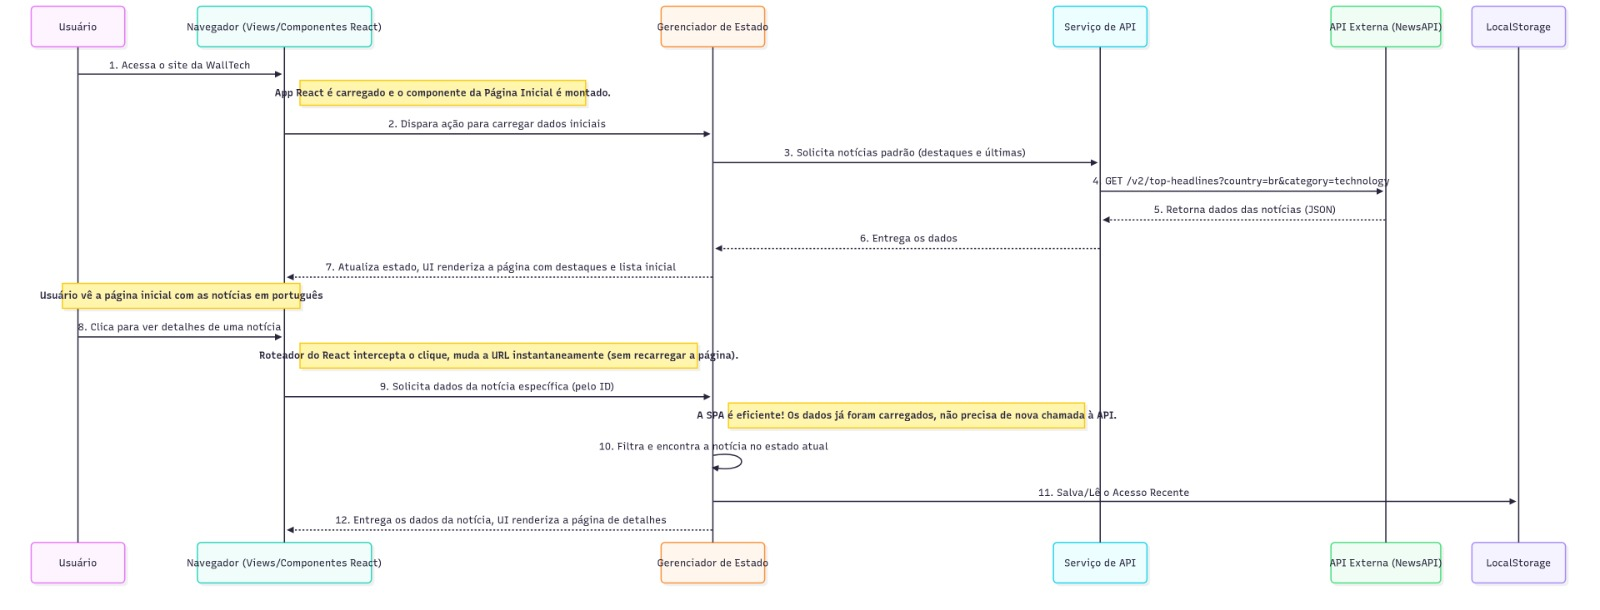
\includegraphics[width=1\textwidth]{media/wall_tech_detail_sequence_diagram.jpeg}
  \legend{Fonte: os autores.}
  \label{fig:sequence-diagram-csr}
\end{figure}


A Figura \ref{fig:component-diagram-react} mostra que, nessa arquitetura, o navegador concentra toda a lógica de renderização. O Roteador React decide quais componentes de página serão exibidos, enquanto o Gerenciador de Estado controla o fluxo de dados entre a interface e a NewsAPI.

\begin{figure}[H]
  \centering
  \caption{Diagrama de Componentes - \acrshort{spa} (React)}
  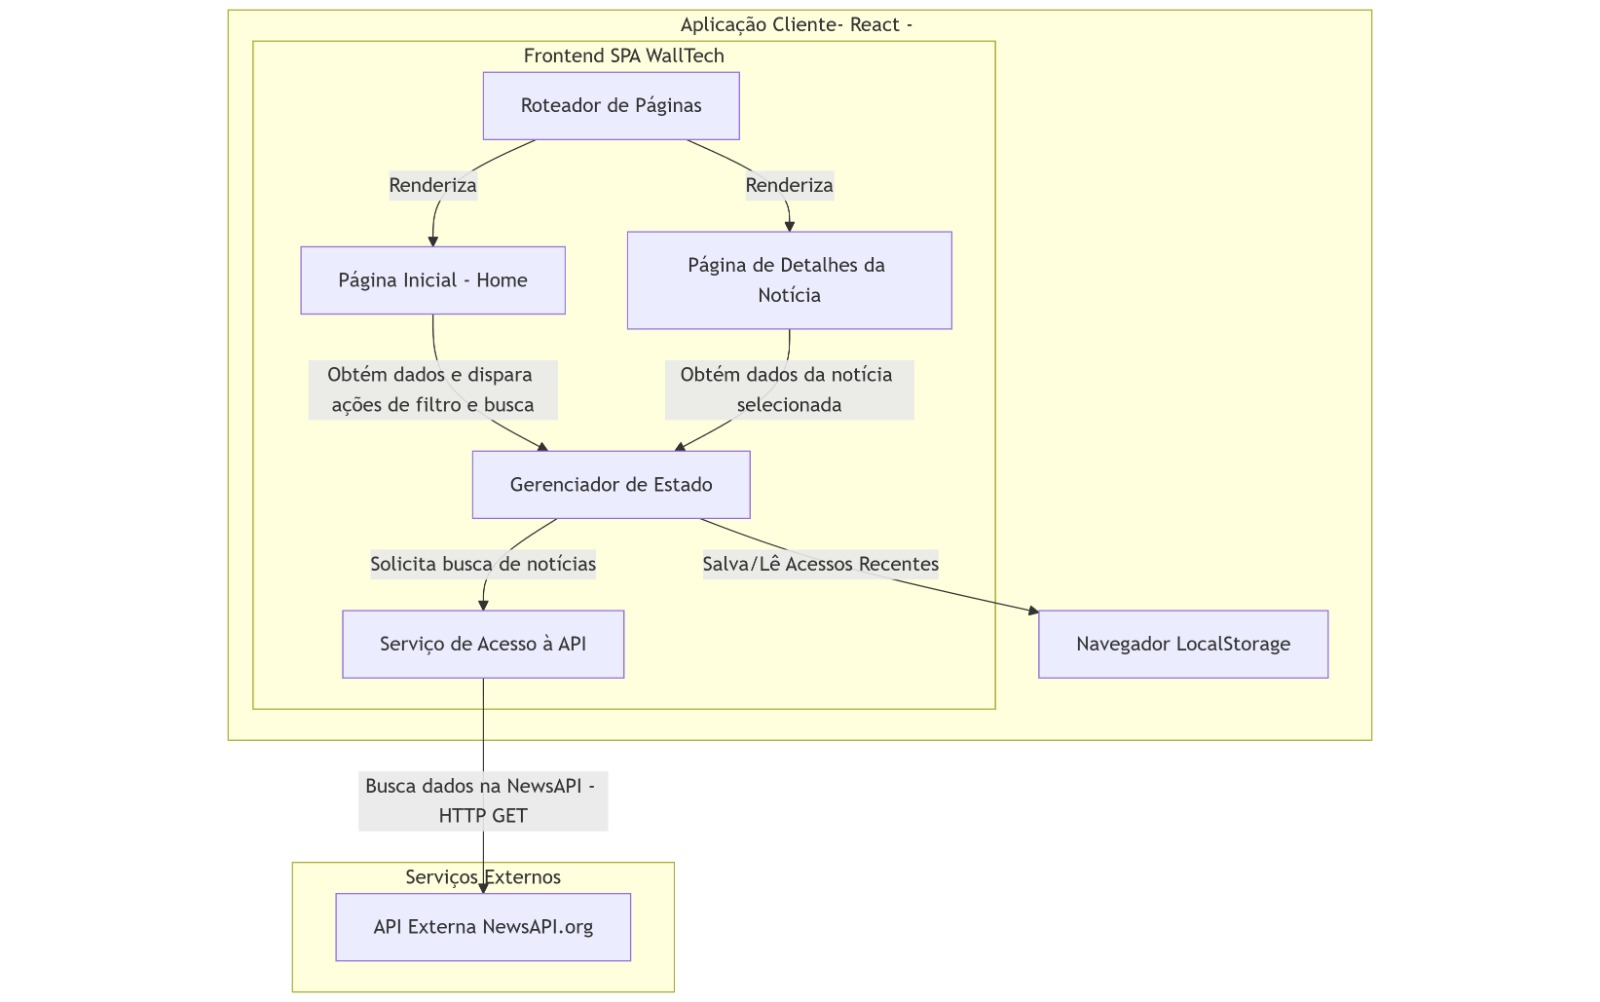
\includegraphics[width=1\textwidth]{media/component-diagram-react.jpeg}
  \legend{Fonte: os autores.}
  \label{fig:component-diagram-react}
\end{figure}



\section{Implementação}
\label{sec:implementacao}

Esta seção descreve o conjunto de tecnologias, bibliotecas e ferramentas que são empregadas para a construção das duas versões do sistema de prova de conceito, detalhando a fundamentação para a escolha de cada componente do ecossistema de desenvolvimento. O gerenciamento do código-fonte e do ciclo de vida do projeto é realizado com o sistema de controle de versão Git e a plataforma de hospedagem GitHub, conforme as práticas descritas na Seção~\ref{sec:git-github}.

Ambas as implementações consomem dados da mesma fonte externa, a News API, uma \acrshort{api} RESTful que fornece o conteúdo jornalístico para a aplicação, como detalhado na Seção~\ref{sec:news-api}. Para garantir a consistência visual e a qualidade da interface entre as duas arquiteturas, utiliza-se a biblioteca de componentes shadcn/ui, que oferece um conjunto de componentes acessíveis e personalizáveis, conforme apresentado na Seção~\ref{sec:ferramentas-modernas}.

\subsection{Implementação da Aplicação SPA}
\label{ssec:implementacao_spa}

A implementação da \acrfull{spa} foi desenvolvida utilizando a biblioteca React na sua versão 18. O React é uma biblioteca JavaScript declarativa, mantida pela Meta, focada na construção de interfaces de usuário a partir de componentes reutilizáveis. Sua adoção neste projeto se dá por sua vasta popularidade no mercado e ao seu paradigma de componentização, que facilita a criação de UIs modulares e de fácil manutenção \cite{react2025}. A eficiência da renderização é otimizada pelo uso de um DOM Virtual, um conceito central da biblioteca que minimiza as manipulações diretas no navegador.

Para a estruturação inicial do projeto e o gerenciamento do ambiente de desenvolvimento, utiliza-se a ferramenta de \textit{build} Vite. O Vite é um ecossistema de desenvolvimento frontend moderno que oferece um servidor de desenvolvimento com recarregamento rápido (\textit{Hot Module Replacement}) e um processo de compilação (\textit{build}) otimizado, que resulta em pacotes de produção menores e mais eficientes \cite{vite_docs}.

O roteamento no lado do cliente, uma característica fundamental da arquitetura SPA, implementa-se com a biblioteca React Router. Trata-se da solução padrão para navegação em aplicações React, que possibilita a criação de uma experiência de usuário fluida e sem recarregamentos de página ao manipular a \acrshort{api} de Histórico do navegador \cite{react_router_docs}. A comunicação com a News API é realizada por meio da \acrshort{api} \texttt{fetch}, nativa dos navegadores modernos.

A \autoref{fig:app-react-csr} mostra a página inicial da plataforma WallTech na implementação \acrshort{spa} com \acrshort{csr}, em conformidade com o wireframe (\autoref{fig:wireframe-walltech}). Nessa página, o usuário visualiza a notícia mais visitada em destaque, três outras recentemente acessadas ao lado, uma lista com as cinco últimas notícias publicadas, além de barra de pesquisa e filtro por país (Brasil ou EUA).

\begin{figure}[H]
  \centering
  \caption{Aplicação SPA com React (\acrshort{csr})}
  
\includegraphics[width=0.9\textwidth]{media/app_react_csr.png}
  \legend{Fonte: os autores.}
  \label{fig:app-react-csr}
\end{figure}

\subsection{Implementação da Aplicação MPA}
\label{ssec:implementacao_mpa}

A implementação da \acrfull{mpa}, com foco em \acrfull{ssr}, é desenvolvida com o \emph{framework} Next.js na versão 14. O Next.js é um meta-framework baseado em React, mantido pela Vercel, que se posiciona como uma solução completa para a construção de aplicações web de produção. Sua escolha para este estudo de caso justifica-se por ser a principal referência de mercado para a implementação de \acrshort{ssr} no ecossistema React, oferecendo uma estrutura robusta e opinativa \cite{nextjs2024}.

O \emph{framework} opera sobre um ambiente Node.js, o que permite a execução de código JavaScript no lado do servidor \cite{nodejs2025}. Essa capacidade é a base da renderização no servidor, onde o Next.js utiliza funções específicas, como a \texttt{getServerSideProps}, para buscar dados de fontes externas e pré-renderizar o HTML completo de uma página antes de enviá-la ao navegador. Além disso, o Next.js implementa um sistema de roteamento baseado no sistema de arquivos, onde a estrutura de diretórios da pasta \texttt{pages} define automaticamente as rotas da aplicação, simplificando a configuração e a manutenção do projeto.


A \autoref{fig:app-next-ssr} mostra a página de detalhes de uma notícia na plataforma WallTech, na implementação \acrshort{mpa} com \acrshort{ssr}. Ao clicar em uma notícia na listagem, o usuário é direcionado para esta tela, onde pode visualizar imagem, fonte, título, metadados (agência e data/hora) e resumo. Também é possível acessar a matéria original pelo botão “Ler na fonte” e retornar à página anterior pelo botão “Voltar”.

\begin{figure}[H]
  \centering
  \caption{Aplicação MPA com Next.js (\acrshort{ssr})}
  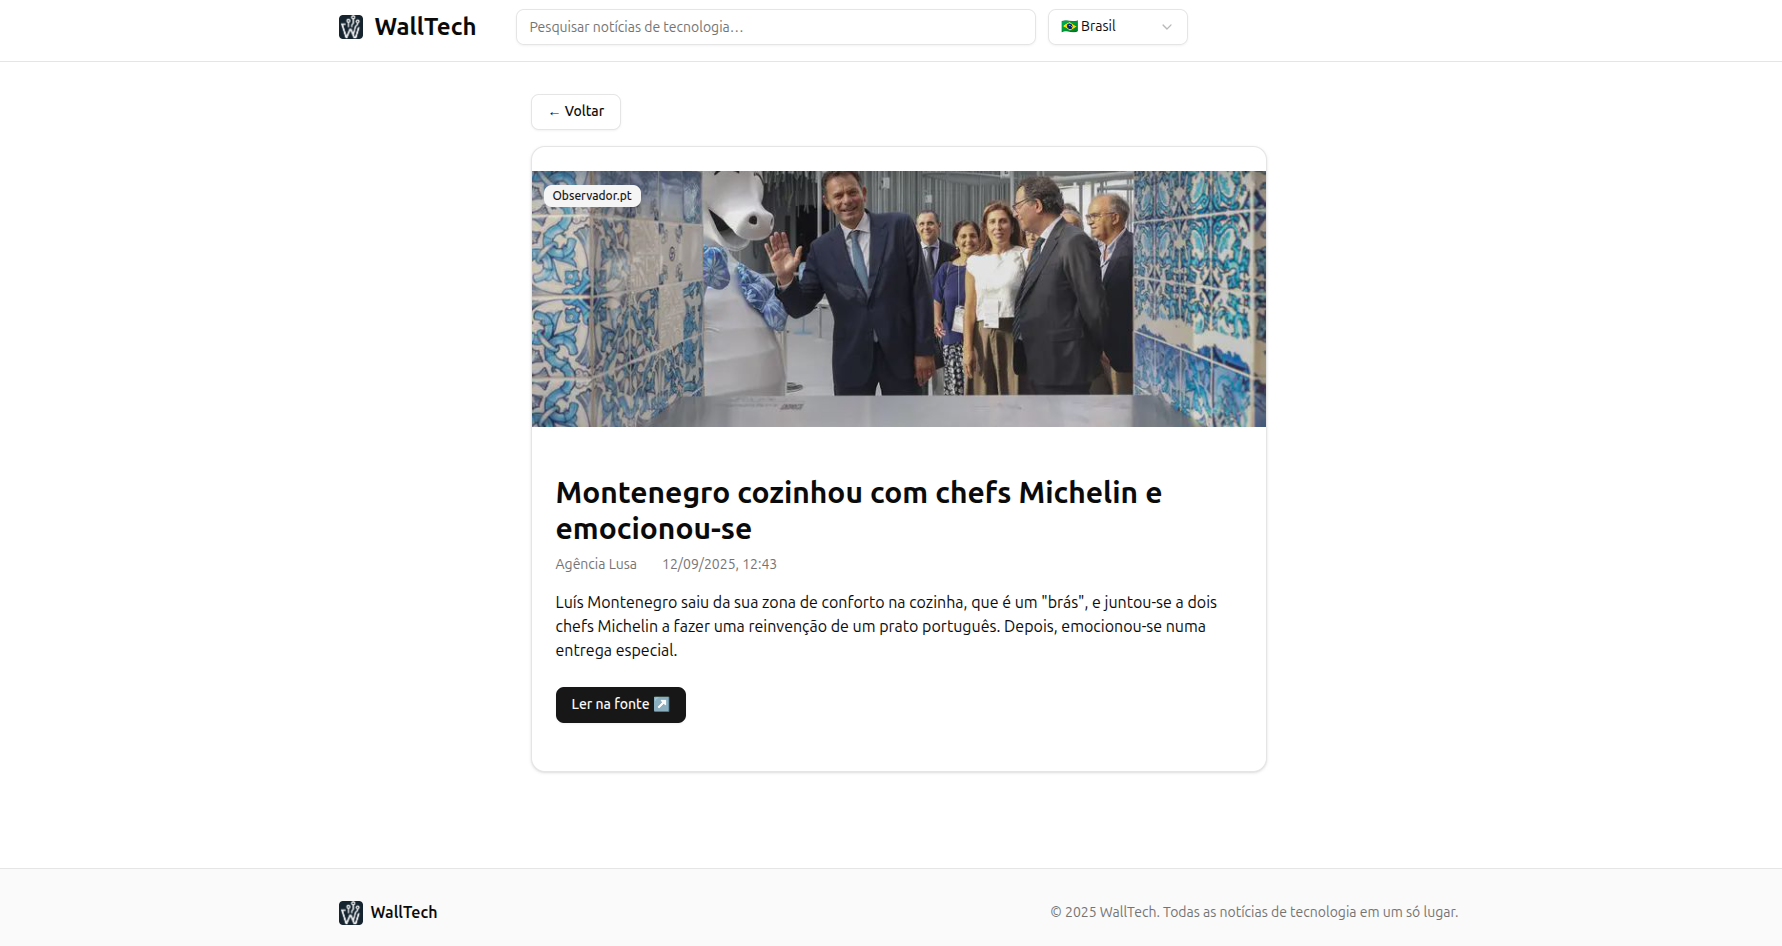
\includegraphics[width=0.9\textwidth]{media/app_next_ssr.png}
  \legend{Fonte: os autores.}
  \label{fig:app-next-ssr}
\end{figure}



\vspace{1cm}
Com as duas versões da plataforma WallTech implementadas e funcionais, o alicerce para a análise comparativa foi estabelecido. O capítulo seguinte detalha o protocolo experimental empregado para a execução dos testes, a configuração do ambiente controlado e os procedimentos de coleta de dados, garantindo que a comparação entre as abordagens \acrshort{csr} e \acrshort{ssr} seja precisa e reprodutível.



\chapter{Coleta de Dados}
\label{cap:metodologia_experimental}


Com as duas versões da plataforma WallTech desenvolvidas, este capítulo descreve o processo prático de coleta de dados que fundamenta a análise de desempenho comparativa. O objetivo é detalhar o ambiente de testes controlado, as ferramentas de instrumentação, o empacotamento das aplicações e os protocolos de execução utilizados. A padronização e o detalhamento dessas etapas são fundamentais para assegurar a validade, a confiabilidade e a reprodutibilidade dos dados que serão apresentados no capítulo de Resultados.



\section{Configuração do Ambiente Experimental}
\label{sec:ambiente-experimental}

Esta seção detalha como as duas versões da plataforma WallTech uma \acrshort{mpa} com \acrshort{ssr} (Next.js) e uma \acrshort{spa} com \acrshort{csr} (React+Vite) foram instrumentadas para coleta de \textit{Web Vitals}, empacotadas em contêineres \textit{Docker} com paridade de recursos e executadas em ambiente local controlado para assegurar reprodutibilidade do estudo.

\subsection{Limitações de Execução e Decisão Metodológica}
\label{ssec:limitacoes-execucao}

Durante o desenvolvimento, a \textit{NewsAPI} impôs restrições de uso em produção (por exemplo, políticas de CORS e/ou limitações do plano vigentes no período do estudo), o que impactaria a coleta de dados em ambiente hospedado. Para eliminar interferências externas e garantir controle experimental, decidiu-se executar ambos os protótipos localmente em contêineres \textit{Docker}, com os mesmos limites de CPU e memória, sistema de arquivos \textit{read-only} e partições temporárias (\textit{tmpfs}) para reduzir variações de I/O. Assim, a comparação \acrshort{csr}~vs.~\acrshort{ssr} foca no \textit{modelo de renderização} e não em diferenças de \textit{hosting}.

\subsection{Instrumentação de Web Vitals}
\label{ssec:instrumentacao-webvitals}

Em ambos os protótipos, a instrumentação é realizada no cliente, e os dados são enviados para um endpoint interno exposto pelo próprio contêiner. Utiliza-se \texttt{navigator.sendBeacon} como via principal (por não bloquear a navegação) e \texttt{fetch} como \textit{fallback} com \texttt{keepalive}. As métricas coletadas são os \textit{Core Web Vitals} atuais: \acrshort{ttfb}, \acrshort{fcp}, \acrshort{lcp}, \acrshort{cls} e \acrshort{inp}.

Os registros são persistidos em NDJSON (uma linha por métrica), contendo, dentre outros, os campos:
\texttt{\{id, name, value, rating, navigationType, attribution, entries, ts\}}. A análise estatística (p.\,ex., p50/p95) está \textit{deliberadamente breve} aqui e será desenvolvida em capítulos posteriores.

Na versão \acrshort{ssr} (App Router), um \textit{Client Component} global usa \texttt{useReportWebVitals} para escutar e enviar as métricas ao endpoint \texttt{/api/vitals}. No servidor, a rota grava o NDJSON em um caminho configurável: por padrão \texttt{/tmp/webvitals.ndjson} (partição \textit{tmpfs}), ou no caminho definido por \texttt{\$METRICS\_PATH} quando se deseja persistência via volume.

\begin{lstlisting}[language=TypeScript,caption={Endpoint de métricas no SSR/Next.js (visão de servidor)}]
// src/app/api/vitals/route.ts
import { NextRequest, NextResponse } from "next/server";
import { appendFile } from "node:fs/promises";

export const runtime = "nodejs";
export const dynamic = "force-dynamic";

const filePath = process.env.METRICS_PATH ?? "/tmp/webvitals.ndjson";

export async function POST(req: NextRequest) {
  const metric = await req.json();
  const doc = { ...metric, ts: new Date().toISOString() };
  await appendFile(filePath, JSON.stringify(doc) + "\n", "utf8");
  return NextResponse.json({ ok: true });
}
\end{lstlisting}

\begin{lstlisting}[language=TypeScript,caption={Envio de métricas no cliente (SSR/Next.js)}]
"use client";
import { useReportWebVitals } from "next/web-vitals";
import { useCallback } from "react";

export default function WebVitals() {
  const report = useCallback((metric: any) => {
    const body = JSON.stringify({
      id: metric.id, name: metric.name, value: metric.value,
      rating: metric.rating, navigationType: metric.navigationType,
      attribution: metric.attribution, entries: metric.entries, ts: Date.now(),
    });

    if (navigator.sendBeacon) {
      navigator.sendBeacon("/api/vitals",
        new Blob([body], { type: "application/json" }));
    } else {
      fetch("/api/vitals", {
        method: "POST", body, keepalive: true,
        headers: { "Content-Type": "application/json" },
      });
    }
  }, []);

  useReportWebVitals(report);
  return null;
}
\end{lstlisting}

Na versão \acrshort{csr}, a coleta usa \texttt{web-vitals/attribution} (para enriquecer \textit{attribution} em \acrshort{lcp}/\acrshort{cls}/\acrshort{inp}). O envio é feito para \texttt{/api/web-vitals}. Como não há servidor \textit{framework} (p.\,ex., Next), a aplicação é servida por um processo Node.js simples (\texttt{server.cjs}) que entrega o \texttt{dist/} e expõe o endpoint de métricas, gravando no mesmo esquema (\texttt{/tmp} ou \texttt{\$METRICS\_PATH}).

\begin{lstlisting}[language=TypeScript,caption={Envio de métricas no cliente (CSR/React+Vite)}]
import { useEffect } from "react";
import { onCLS, onINP, onLCP, onFCP, onTTFB, type MetricWithAttribution } from "web-vitals/attribution";

export default function WebVitals() {
  useEffect(() => {
    const report = (m: MetricWithAttribution) => {
      const body = JSON.stringify({
        id: m.id, name: m.name, value: m.value, rating: m.rating,
        navigationType: m.navigationType, attribution: m.attribution,
        entries: m.entries, ts: Date.now(),
      });

      if (navigator.sendBeacon) {
        navigator.sendBeacon("/api/web-vitals",
          new Blob([body], { type: "application/json" }));
      } else {
        fetch("/api/web-vitals", {
          method: "POST", body, keepalive: true,
          headers: { "Content-Type": "application/json" },
        });
      }
    };

    onCLS(report); onINP(report); onLCP(report); onFCP(report); onTTFB(report);
  }, []);

  return null;
}
\end{lstlisting}

\begin{lstlisting}[language=Java,caption={Servidor estático + endpoint (CSR/React+Vite)}]
// server.cjs - Node HTTP simples (serve dist/ e expõe /api/web-vitals)
const http = require("node:http");
const { appendFile, readFile, stat } = require("node:fs/promises");
const { createReadStream } = require("node:fs");
const path = require("node:path");

const PORT = process.env.PORT || 3000;
const DIST = path.join(process.cwd(), "dist");
const METRICS_PATH = process.env.METRICS_PATH || "/tmp/webvitals.ndjson";

const server = http.createServer(async (req, res) => {
  const url = new URL(req.url, `http://${req.headers.host}`);

  if (url.pathname === "/api/web-vitals") {
    if (req.method === "POST") {
      const chunks = []; req.on("data", c => chunks.push(c));
      req.on("end", async () => {
        const json = JSON.parse(Buffer.concat(chunks).toString("utf8") || "{}");
        await appendFile(METRICS_PATH, JSON.stringify({ ...json, ts: Date.now() }) + "\n", "utf8");
        res.writeHead(200, { "Content-Type": "application/json" });
        res.end(JSON.stringify({ ok: true }));
      });
      return;
    }
    if (req.method === "GET") {
      const data = await readFile(METRICS_PATH, "utf8").catch(() => "");
      res.writeHead(200, { "Content-Type": "application/x-ndjson" });
      res.end(data); return;
    }
    res.writeHead(405).end(); return;
  }

  // estático + fallback SPA
  let p = decodeURIComponent(url.pathname);
  if (p === "/") p = "/index.html";
  const file = path.join(DIST, p);
  try {
    const s = await stat(file); if (s.isDirectory()) throw 0;
    createReadStream(file).pipe(res);
  } catch {
    createReadStream(path.join(DIST, "index.html")).pipe(res);
  }
});
server.listen(PORT);
\end{lstlisting}

\subsection{Empacotamento Docker: SSR/MPA (Next.js) e CSR/SPA (React+Vite)}
\label{ssec:docker-packaging}

Para a aplicação com \acrshort{ssr}, adotou-se o modo standalone do Next.js e \textit{multi-stage build}: (i) instalação de dependências, (ii) \textit{build} e (iii) \textit{runner} minimalista. O contêiner expõe a porta \texttt{3000}, roda como usuário \texttt{node} e lê variáveis em tempo de execução (importante para segredos e chaves).

\begin{lstlisting}[language=Dockerfile,caption={Dockerfile da aplicação SSR/MPA (Next.js)}]
# ---------- 1) deps ----------
FROM node:20-alpine AS deps
WORKDIR /app
COPY package*.json ./
RUN npm ci --ignore-scripts

FROM node:20-alpine AS builder
WORKDIR /app
ENV NEXT_TELEMETRY_DISABLED=1
COPY --from=deps /app/node_modules ./node_modules
COPY . .
RUN npm run build

FROM node:20-alpine AS runner
WORKDIR /app
ENV NODE_ENV=production
ENV NEXT_TELEMETRY_DISABLED=1

COPY --from=builder /app/.next/standalone ./
COPY --from=builder /app/public ./public
COPY --from=builder /app/.next/static ./.next/static

USER node
EXPOSE 3000
CMD ["node", "server.js"]
\end{lstlisting}

\begin{lstlisting}[language=bash,caption={Build e execução do container SSR com limites e volume de métricas}]
docker build --no-cache -t next-ssr:prod .

docker run --name next-ssr \
  -p 3001:3000 \
  -e METRICS_PATH=/data/webvitals.ndjson \
  -v "$PWD/metrics:/data:rw" \
  --cpus="1.00" --cpuset-cpus="0" \
  --memory="1g" --memory-swap="1g" \
  --pids-limit=256 \
  --read-only \
  --tmpfs /tmp \
  --tmpfs /app/.next/cache \
  next-ssr:prod
\end{lstlisting}

Já para a aplicação com \acrshort{csr}, o \textit{build} é produzido pelo Vite e servido por \texttt{server.cjs}. Diferentemente do \acrshort{ssr}, as variáveis \texttt{VITE\_*} são resolvidas em tempo de build; por isso, a \texttt{.env} é copiada para o estágio \textit{builder} (ou alternativamente injetada com \texttt{--build-arg}). Em execução, o caminho do arquivo de métricas é definido por \texttt{\$METRICS\_PATH}.

\begin{lstlisting}[language=Dockerfile,caption={Dockerfile da aplicação CSR/SPA (React+Vite)}]
# ---------- 1) deps ----------
FROM node:20-alpine AS deps
WORKDIR /app
COPY package*.json ./
RUN npm ci --ignore-scripts

# ---------- 2) build ----------
FROM node:20-alpine AS builder
WORKDIR /app
COPY --from=deps /app/node_modules ./node_modules
COPY . .
# 👇 garante que o Vite leia suas VITE_* do host
COPY .env ./.env
RUN npm run build

# ---------- 3) runner ----------
FROM node:20-alpine AS runner
WORKDIR /app
ENV NODE_ENV=production
ENV TZ=UTC
ENV NODE_OPTIONS=--max-old-space-size=512
COPY --from=builder /app/dist ./dist
COPY server.cjs ./server.cjs
USER node
EXPOSE 3000
CMD ["node", "server.cjs"]
\end{lstlisting}

\begin{lstlisting}[language=bash,caption={Build e execução do container CSR com limites e volume de métricas}]
docker build -t react-csr:prod .

docker run --name react-csr \
  -p 3002:3000 \
  -e METRICS_PATH=/data/webvitals.ndjson \
  -v "$PWD/metrics-csr:/data:rw" \
  --cpus="1.00" --cpuset-cpus="0" \
  --memory="1g" --memory-swap="1g" \
  --pids-limit=256 --read-only --tmpfs /tmp \
  react-csr:prod
\end{lstlisting}

\subsection{Paridade de Recursos, Observabilidade e Procedimento de Coleta}
\label{ssec:paridade-observabilidade}

Para evitar viés de ambiente, ambos os contêineres executam com paridade de recursos: \texttt{--cpus="1.0"}, \texttt{--cpuset-cpus="0"} (fixação na CPU 0), \texttt{--memory="1g"}, \texttt{--memory-swap="1g"}, \texttt{--pids-limit=256}, \texttt{--read-only} e \texttt{--tmpfs /tmp} (arquivo de métricas em memória quando não houver volume). No \acrshort{ssr}, \texttt{/app/.next/cache} é montado em \texttt{tmpfs} para reduzir variações de disco.

Durante os testes, o uso de recursos foi acompanhado com:
\begin{lstlisting}[language=bash]
docker stats next-ssr
docker stats react-csr
\end{lstlisting}
Esse monitoramento fornece CPU\% e memória em tempo real, complementando a coleta de \textit{Web Vitals}. O procedimento adotado foi:
(i) \textit{warm-up} com 2 acessos iniciais à mesma rota para estabilizar caches;
(ii) coleta de 10--15 carregamentos por cenário (janela anônima);
(iii) persistência NDJSON por cenário em volumes distintos (por exemplo, \texttt{./metrics} para \acrshort{ssr} e \texttt{./metrics-csr} para \acrshort{csr}).
A análise de métricas (estatísticas descritivas e percentis como p50 e p95) será apresentada em capítulo específico.

\subsection{Repositórios e Reprodutibilidade}
\label{ssec:repositorios-repro}
O código-fonte, instruções de execução e artefatos de instrumentação estão disponíveis nos repositórios públicos da empresa fictícia WallTech:
\begin{itemize}
  \item \textbf{CSR/SPA (React+Vite)}: \url{https://github.com/WallTechTCC/React-CSR}
  \item \textbf{SSR/MPA (Next.js)}: \url{https://github.com/WallTechTCC/Next-SSR}
\end{itemize}
Esses repositórios permitem reproduzir o experimento localmente com os mesmos limites de CPU/RAM, sistema de arquivos \textit{read-only} e coleta de \textit{Web Vitals} no formato NDJSON, preservando a comparabilidade entre \acrshort{csr} e \acrshort{ssr}.


\subsection{Coleta de CPU/RAM do contêiner e exportação em CSV}
\label{ssec:coleta-host-docker-stats}

Para registrar o uso de CPU, memória e número de \textit{PIDs} dos contêineres durante os cenários de teste, foi utilizada a telemetria do próprio Docker via \texttt{docker stats} (sem streaming contínuo). As amostras foram coletadas a cada 1 segundo e gravadas em arquivos CSV separados por aplicação, no diretório \texttt{metrics-host/}.

Cada linha do arquivo CSV gerado contém as seguintes colunas para a análise dos dados:
\begin{itemize}
  \item \textbf{ts}: timestamp da coleta no host (\texttt{YYYY-MM-DD HH:MM:SS});
  \item \textbf{name}: nome do contêiner;
  \item \textbf{cpu\_perc}: percentual de CPU do contêiner (string com ``\%'' conforme \texttt{docker stats});
  \item \textbf{mem\_usage}: uso de memória reportado (formato humano, ex.: ``123.4MiB / 1.00GiB'');
  \item \textbf{mem\_perc}: percentual de memória (string com ``\%'');
  \item \textbf{pids}: quantidade de processos/threads visíveis ao cgroup do contêiner.
\end{itemize}

O comando utilizado para a coleta no contêiner \textbf{SSR (\texttt{next-ssr})}, que cria o diretório de métricas e inicia a captura contínua em \texttt{metrics-host/docker-stats-ssr.csv}, é apresentado a seguir.

\begin{lstlisting}[language=bash,caption={Captura de CPU/RAM do contêiner SSR e exportação para CSV}]
mkdir -p metrics-host
(
  echo "ts,name,cpu_perc,mem_usage,mem_perc,pids";
  while true; do
    TS=$(date +"%F %T");
    docker stats --no-stream \
      --format "{{.Name}},{{.CPUPerc}},{{.MemUsage}},{{.MemPerc}},{{.PIDs}}" \
      next-ssr | sed "s/^/$TS,/";
    sleep 1;
  done
) >> metrics-host/docker-stats-ssr.csv
\end{lstlisting}

De forma análoga, a coleta para o contêiner \textbf{CSR (\texttt{react-csr})} foi realizada com o script abaixo, gravando os dados em \texttt{metrics-host/docker-stats-csr.csv}.

\begin{lstlisting}[language=bash,caption={Captura de CPU/RAM do contêiner CSR e exportação para CSV}]
(
  echo "ts,name,cpu_perc,mem_usage,mem_perc,pids";
  while true; do
    TS=$(date +"%F %T");
    docker stats --no-stream \
      --format "{{.Name}},{{.CPUPerc}},{{.MemUsage}},{{.MemPerc}},{{.PIDs}}" \
      react-csr | sed "s/^/$TS,/";
    sleep 1;
  done
) >> metrics-host/docker-stats-csr.csv
\end{lstlisting}

\subsection{Uso complementar do Lighthouse (Chrome DevTools)}
\label{ssec:lighthouse}

O \textit{Lighthouse} foi utilizado como apoio diagnóstico em ambiente laboratorial, para identificar gargalos e oportunidades que expliquem diferenças observadas nas medições de campo.

No contexto deste estudo, o Lighthouse foi empregado com os seguintes propósitos:
\begin{itemize}
  \item \textbf{Interatividade em laboratório}: leitura do TBT (\textit{Total Blocking Time}) como indicador de trabalho bloqueante no \textit{main thread};
  \item \textbf{Oportunidades/Auditorias}: insumos para orientar correções de build e de carregamento (JS/CSS, imagens, dicas de rede);
  \item \textbf{Acessibilidade e SEO}: verificação rápida de barreiras e sinalização para mecanismos de busca.
\end{itemize}

Os testes foram executados no Google Chrome, em \textit{DevTools} \textrightarrow{} Lighthouse, no modo \textit{Navigation}, com throttling padrão de rede/CPU, em \textit{Mobile} e, quando pertinente, \textit{Desktop}. Para cada cenário (página inicial, resultados de busca, detalhes da notícia) foram feitas 3 execuções, registrando-se a mediana do TBT e as principais oportunidades reportadas. Os relatórios foram exportados em JSON e HTML.

Na análise de performance, priorizou-se:
\begin{itemize}
  \item \acrshort{tbt} (\textit{numericValue} e evidências de \textit{long tasks});
  \item \textbf{Oportunidades e auditorias} diretamente relacionadas a custo de carregamento e execução:
  \begin{itemize}
    \item \textit{render-blocking-resources};
    \item \textit{unused-javascript} e \textit{unused-css-rules};
    \item \textit{total-byte-weight} e \textit{legacy-javascript};
    \item \textit{mainthread-work-breakdown} e \textit{diagnostics};
    \item \textit{modern-image-formats}, \textit{uses-text-compression}, \textit{preload}, \textit{preconnect}.
  \end{itemize}
\end{itemize}

Na parte de acessibilidade, foram verificados itens que impactam navegação por teclado, leitores de tela e clareza de interface:
\begin{itemize}
  \item \textbf{Semântica e estrutura}: hierarquia de \textit{headings} e \textit{landmarks} (banner, main, nav);
  \item \textbf{Foco e tabulação}: ordem lógica, foco visível, ausência de \textit{focus traps};
  \item \textbf{Rótulos e nomes acessíveis}: uso adequado de \texttt{label} e atributos \texttt{aria-*};
  \item \textbf{Contraste e legibilidade}: verificação de contraste de cor e tamanhos de fonte;
  \item \textbf{Alternativos de mídia}: textos alternativos em imagens e propósito claro de links/botões.
\end{itemize}
Dos relatórios JSON, foram lidos os \texttt{audits} mais acionáveis, como
\texttt{color-contrast}, \texttt{image-alt}, \texttt{label}, \texttt{link-name},
\texttt{heading-order}, \texttt{landmark-one-main}, \texttt{focus-traps} e \texttt{logical-tab-order}.

A verificação de \acrshort{seo} concentrou-se em sinalização técnica e rastreabilidade:
\begin{itemize}
  \item \textbf{Sinalização}: título e meta description presentes; \texttt{rel=canonical} consistente;
  \item \textbf{Rastreabilidade}: links rastreáveis, \texttt{robots.txt}/meta robots válidos;
  \item \textbf{Internacionalização e dados estruturados}: \texttt{hreflang} (quando aplicável) e \textit{structured data} sem erros;
  \item \textbf{Compatibilidade móvel}: viewport configurado, fontes legíveis e \textit{tap targets} adequados.
\end{itemize}
Foram consultados, entre outros, os \texttt{audits}: \texttt{document-title}, \texttt{meta-description}, \texttt{canonical}, \texttt{is-crawlable}, \texttt{robots-txt}, \texttt{hreflang}, \texttt{structured-data}, \texttt{viewport}, \texttt{font-size} e \texttt{tap-targets}.

Os relatórios foram versionados com convenção por cenário (\textit{ex.}, \texttt{lighthouse\_csr\_home\_mobile\_run\_1.json}). Do JSON, foram consumidos apenas campos necessários para explicar diferenças observadas nos resultados de campo e para orientar correções de implementação.

Resultados do Lighthouse são laboratoriais, dependentes de emulação de CPU/rede e do ambiente local do avaliador. Por isso, são utilizados como indícios de causa e para priorização de melhorias, e não como substitutos das medições coletadas em execução real.
